The goal of our study is to understand technical debt found in source code comments. To do so, we first manually analyze the comments identifying technical debt comments in the selected projects. We divide our research question in two parts first, we classify the comments into technical debt types accordingly with their nature. Second, we quantify these comments identifying the most common types of self-admitted technical debt. In the remainder of this section we detail the motivation, approach and results for our research question.  

\vspace{3mm}
\noindent\rqi
\vspace{3mm}

\noindent\textbf{Motivation:} As shown in previous work \cite{Potdar2014ICSME}, self-admitted technical can be an indicator of non-optimal solutions. However, technical debt is a general term, and there are many different types of technical debt \cite{Alves2014MTD}. Although we know that self-admitted technical exists, the different kinds of self-admitted technical debt is still  unknown. Answering this question is important as different types of debt has different approaches to be solved, and therefore each different type may need a tailored solution. 

\vspace{1mm}
\noindent\textbf{Approach:} To identify the different types of debt found in the comments we manually read trough all filtered comments as described in Section \ref{sec:approach}. While examining the comments we classify each comment by the nature of the debt as proposed by Alves \textit{et al.} in previous work. 

During the classification we notice that some comments can be classified in more than one type of debt (e.g., A comment reporting a Design Debt can also means that a particular piece of code is causing an unexpected behavior, which is a Defect Debt). Although this is an ambiguous situation, and may have different interpretations depending of who is reading the comments, we defined that each comment would have just one classification type for the sake of clarity. To mitigate the chance of misclassifying these comments, we take in consideration the more meaningful type for each comment in a given scenario. To do so, a more detail investigation was necessary (i.e., looking at the source code). In total we read and classified 33,093 comments from five open source projects. The classification took approximately 85 hours and was performed by the first author of the paper. 

\vspace{1mm}
\noindent\textbf{Results:} First, we present the types of self-admitted technical debt that we could find in the source code comments that we classified. 

\begin{itemize}
  \item \textbf{Self-admitted Design debt:} These comments indicates that there is a problem with the design of the code. They can be comments about misplaced code, lack of abstraction, long methods, poor implementation, workarounds and temporary solution were classified in this type. Lets consider the following comments:
  
  \vspace{1mm}
  \begin{displayquote}
     \textit{``TODO: - This method is too complex, lets break it up''}
     
     \vspace{1mm}

     \textit{``/* TODO: really should be a separate class */''}
  \end{displayquote}
  \vspace{1mm}

  These comments are clear examples of what we consider a self-admitted design debt. The authors states their analysis and what need to be done in order to improve the current design of the code. Although, during the analysis we came across more challenging comments that expressed design problems in an indirect way:  
  
  \vspace{1mm}
  \begin{displayquote}
     \textit{``// I hate this so much even before I start writing it. // Re-initialising a global in a place where no-one will see it just // feels wrong.  Oh well, here goes.''}

     \vspace{1mm}

     \textit{``//quick \& dirty, to make nested mapped p-sets work:''}
  \end{displayquote}
  \vspace{1mm}

  In the above examples the authors are certain to be implementing code that does not represent the best solution. Intuitively, we know that kind of implementation will degrade the design of the code and should be avoided. 

  \vspace{1mm}
  \begin{displayquote}
      \textit{``// probably not the best choice, but it solves the problem of // relative paths in CLASSPATH''}

      \vspace{1mm}

      \textit{``//I can't get my head around this; is encoding treatment needed here?''}
  \end{displayquote}
  \vspace{1mm}

  The above comments expressed doubt and uncertainty when implementing the code and were considered as self-admitted design debt as well.

  \item \textbf{Self-admitted Defect debt:} In defect debt comments the author states that a particular piece of code do not have the expected behavior, meaning that there is a defect in the code. 
  
  \vspace{1mm}
  \begin{displayquote}
      \textit{``// Bug in above method''}

      \vspace{1mm}

      \textit{``// WARNING: the OutputStream version of this doesn't work!''}
  \end{displayquote}
  \vspace{1mm}
  
  As shown in these examples there are defects that are known by the developers, but for some reason is not fixed yet. 

  \item \textbf{Documentation debt:} In the documentation debt comments the author express that there is not proper documentation supporting that part of the program.
  
  \vspace{1mm}
  \begin{displayquote}
  	\textit{``**FIXME** This function needs documentation''}
  	
  	\vspace{1mm}
  	
  	\textit{``// TODO Document the reason for this''}
  \end{displayquote}
  \vspace{1mm}
  
  \item \textbf{Self-admitted Requirement debt:} Requirement debt comments express incompleteness of the method, class or program.
  
  \begin{displayquote}
  	\textit{``/TODO no methods yet for getClassname''}
  	
  	\vspace{1mm}
  	
  	\textit{``//TODO no method for newInstance using a reverse-classloader''}

  	\vspace{1mm}
  	
  	\textit{``TODO: The copy function is not yet * completely implemented - so we will  * have some exceptions here and there.*/''}  
  	
  \end{displayquote}
  \vspace{1mm}  
  
  	The last example shows a comment that could be considered as having more than one type of debt. (i.e., requirement debt and defect debt), but as mentioned in the classification approach, we choose to maintain one type only for each comment. 
  	
  	In our understanding, the defect debt expressed in the comment would not exist if the requirement debt did not exists. Therefore, the main debt in this comment is a requirement debt (i.e., incomplete implementation of the copy function). 
  	
  	One more reason that we give a comment only one classification type is that there is no way to tell if the other requirement debts are not causing an unexpected behavior, except in the case that the author of the comment express is. 
  
  \vspace{1mm}
  \item \textbf{Self-admitted Test debt:} Test debt comments are the ones that express the need for implementation or improvement of the current tests. As shown in the examples below, test debt comments are very straight forward in their meaning. 
  
  \begin{displayquote}
  	\textit{``// TODO - need a lot more tests''}
  	
  	\vspace{1mm}
  	
  	\textit{``//TODO enable some proper tests!!''}
  \end{displayquote}
  \vspace{1mm}  
    
\end{itemize}

After classifying the comments, we notice that not all of the types mentioned in \cite{Alves2014MTD} could be found. We argue that some of the types like People Debt or Infrastructure Debt is really less probable to appear in source code comments, whereas other types as Build Debt could not be found because we are examining just comments found in Java classes, therefore not taking in consideration build scripts that can be written in other languages (e.g., Maven and Ant use XML files as build scripts). 

Other than that, types like Test Automation debt and Test Debt were considered as the same type in our study due to the resemblance of their purpose. In a similar way, Process Debt, Service Debt, Code Debt and Architecture Debt were considered as Self-admitted design debt in our study.

\conclusionbox{We found 5 different types of self-admitted technical debt in the comments of the studied projects. Design Debt, Defect Debt, Documentation Debt, Requirement Debt and Test Debt. Althoug there are comments that can have more the one type of debt, we found that there is a main type of debt that the comment can be classified to. }

\begin{figure*}[thb!]
  \caption{Self-admitted technical debt types distribution}
  \centering
  \label{fig:satd_distribution}
  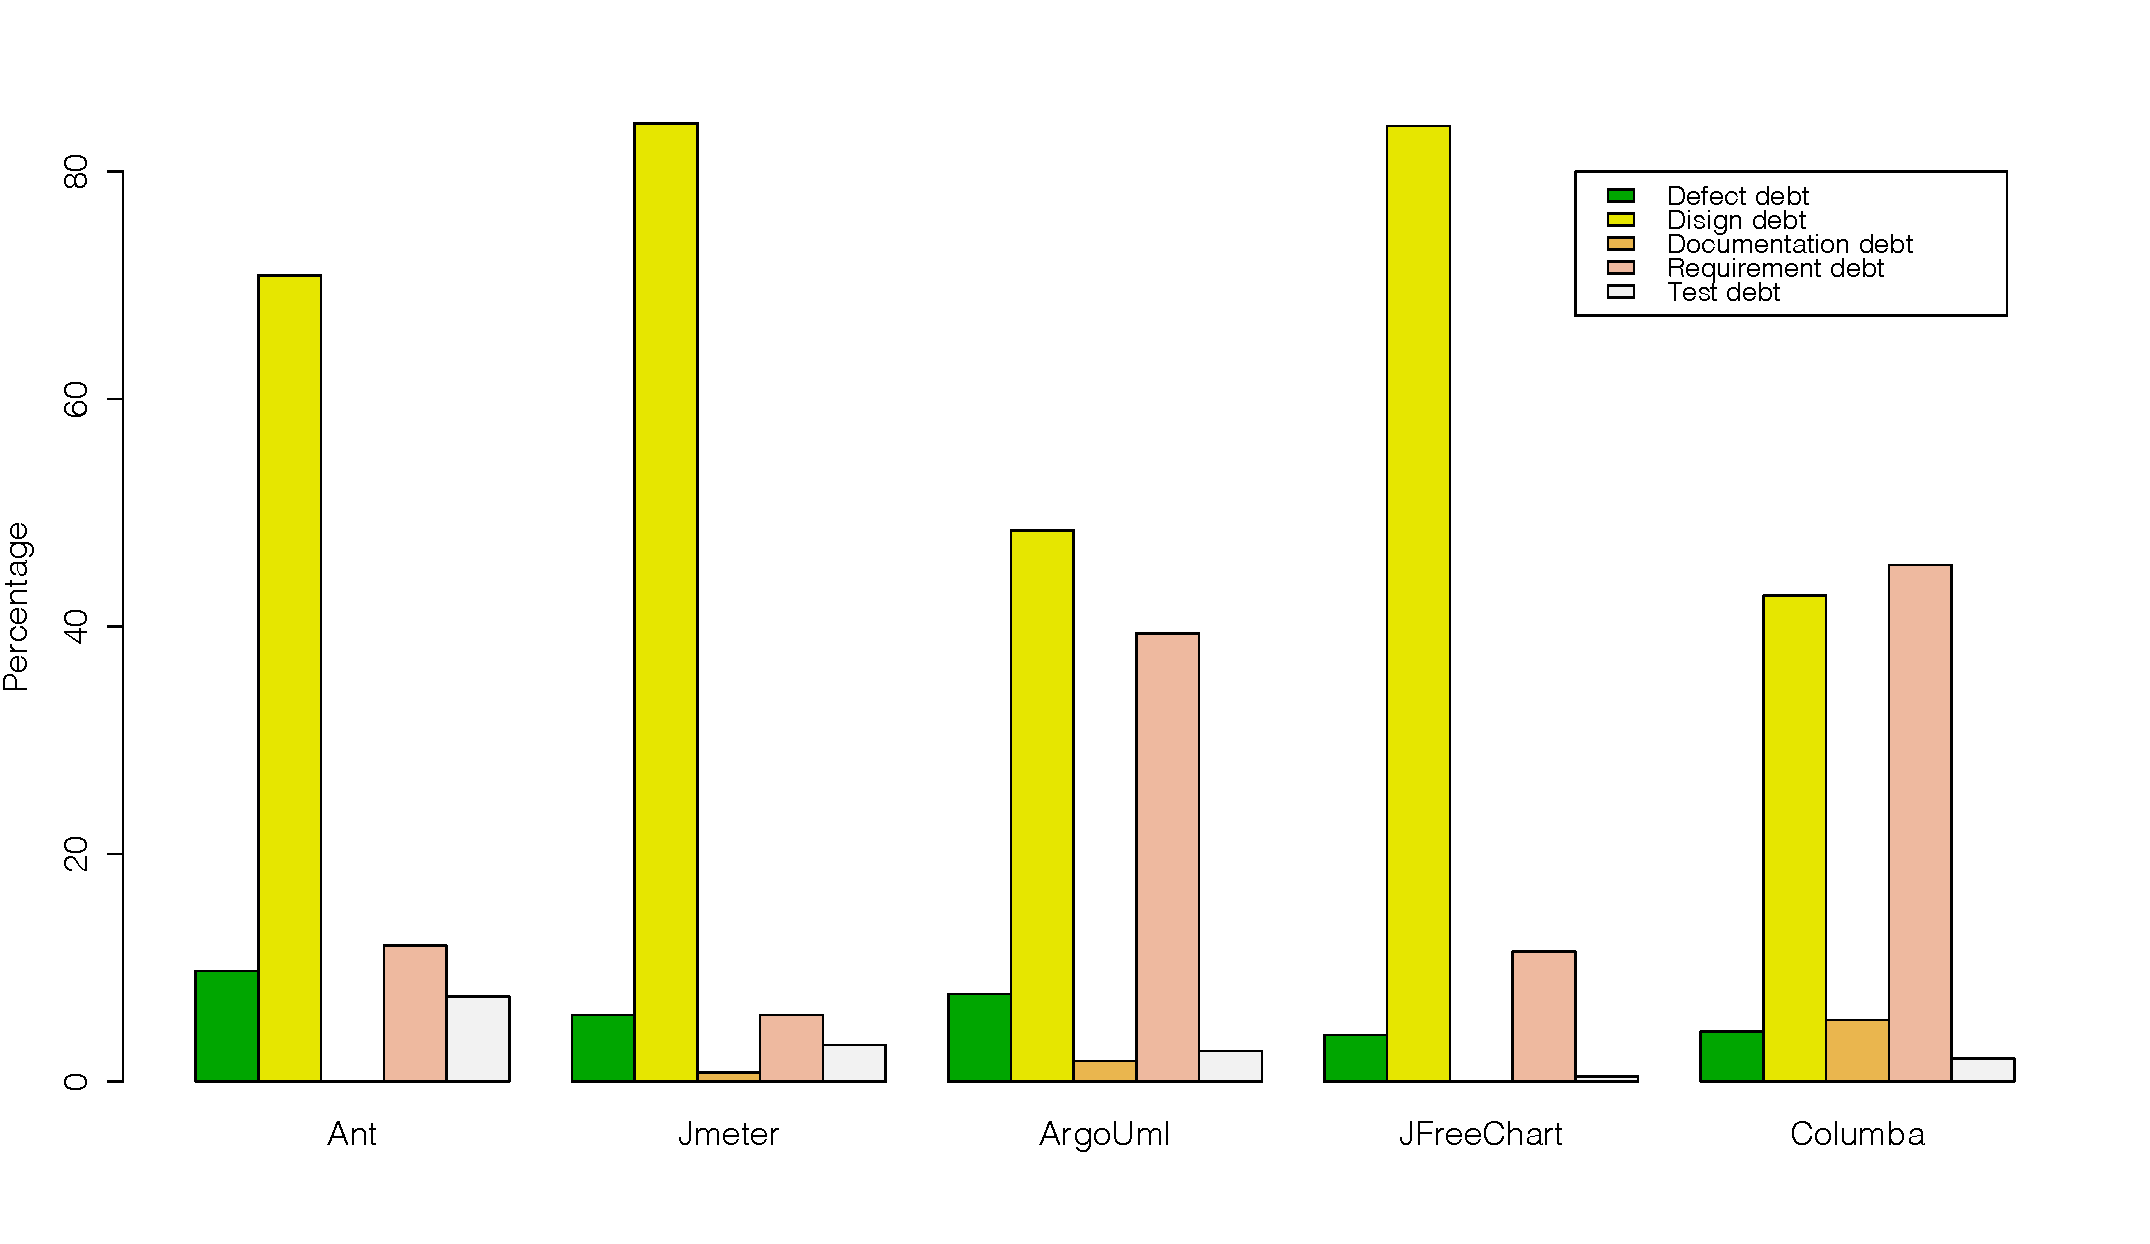
\includegraphics[width=1\textwidth]{figures/technical_debt_distribution.pdf}
\end{figure*}

% Table \ref{tab:technical_debt_project} shows the total amount of self-admitted technical debt found in the analyzed projects. For example, in Apache Ant out of the 4,140 analyzed comments 134 turnout to be classified as self-admitted technical debt, which represents 3.2\% of the comments of the analyzed comments. 

% Analyzing the results of the classification we found that the comments could be classified in one of the following types of debt: design debt, defect debt, documentation debt, requirement debt and  test debt. 
 
% To a comment be classified as design debt it has to indicate that there is a problem with design of the code (e.g., misplaced code, lack of abstraction, long method, poor implementation). Table \ref{tab:design_debt_detail} show some concrete examples of the comments classified as Design Debt. 

% In defect debt comments the author/s states that that particular piece of code do not have the expected behavior. For documentation debt comments the author/s wrote that there is not documentation supporting that part of the program. Requirement debt comments express the fact that incompleteness of the method, class or program. Finally, test debt comments are the ones that express the need for implementation or improvement of the current tests. We show examples of defect, documentation, requirement and test debt in Tables \ref{tab:defect_debt_detail}, \ref{tab:documentation_debt_detail}, \ref{tab:requeriment_debt_detail}, \ref{tab:test_debt_detail} respectively.   

%\begin{table*}[!hbt]
%      \begin{center}
%            \caption{Self-admitted technical debt per project}
%            \label{tab:technical_debt_project}
%            \begin{tabular}{l| c c c }
%            \toprule
%            \textbf{Project}      & \textbf{Analyzed comments}     & \textbf{Self-admitted TD comments} & \textbf{Percentage} \\ \midrule 
%              Apache Ant          & 4,140                          & 134                                & 3.2  \\                                   
%              Apache Jmeter       & 8,163                          & 375                                & 4.6  \\                                   
%              ArgoUML             & 9,788                          & 1,653                              & 16.8 \\                                   
%              Columba             & 6,569                          & 295                                & 4.4 \\                                   
%              JFreeChart          & 4,433                          & 219                                & 4.9  \\ \bottomrule
%            \end{tabular}
%      \end{center}
%\end{table*}

% \begin{table}[!hbt]
%       \begin{center}
%             \caption{Self-admitted design technical debt examples}
%             \label{tab:design_debt_detail}
%             \begin{tabular}{l}
%             \toprule
%             \textbf{Comments}     \\ \midrule 
%              // XXX Move to Project ( so it is shared by all helpers ) \\                                   
%              // XXX maybe use reflection to addPathElement (other patterns ?) \\                                   
%              // TODO: move this to components \\                                   
%              // Can be written better... this is too hacky! \\                                   
%              // Yuck: TIFFImageEncoder uses Error to report runtime problems \\ \bottomrule
%             \end{tabular}
%       \end{center}
% \end{table}

% \begin{table}[!hbt]
%       \begin{center}
%             \caption{Self-admitted defect technical debt examples}
%             \label{tab:defect_debt_detail}
%             \begin{tabular}{l}
%             \toprule
%             \textbf{Comments}     \\ \midrule 
%              // FIXME formatters are not thread-safe\\                                   
%              // Bug in above method \\                                   
%              // TODO: This does not work! (MVW)\\                                   
%              // WARNING: the OutputStream version of this doesn't work!\\                                   
%              // TODO: This looks backwards. Left over from issue 2034? \\ \bottomrule
%             \end{tabular}
%       \end{center}
% \end{table}

% \begin{table}[!hbt]
%       \begin{center}
%             \caption{Self-admitted documentation technical debt examples}
%             \label{tab:documentation_debt_detail}
%             \begin{tabular}{l}
%             \toprule
%             \textbf{Comments}     \\ \midrule 
%             // **FIXME** This function needs documentation\\                                   
%             // TODO Document the reason for this\\                                   
%             // TODO: Document exceptional behaviour.\\                                   
%             // TODO: centralise this knowledge.\\  \bottomrule
%             \end{tabular}
%       \end{center}
% \end{table}

% \begin{table}[!hbt]
%       \begin{center}
%             \caption{Self-admitted requirement technical debt examples}
%             \label{tab:requeriment_debt_detail}
%             \begin{tabular}{l}
%             \toprule
%             \textbf{Comments}     \\ \midrule 
%             // TODO: not implemented\\                                   
%             // TODO Auto-generated constructor stub\\                                   
%             // TODO: i18n\\                                   
%             // TODO no methods yet for getClassname  \\                                   
%             // TODO no method for newInstance using a reverse-classloader \\ \bottomrule
%             \end{tabular}
%       \end{center}
% \end{table}

% \begin{table}[!hbt]
%       \begin{center}
%             \caption{Self-admitted test technical debt examples}
%             \label{tab:test_debt_detail}
%             \begin{tabular}{l}
%             \toprule
%             \textbf{Comments}     \\ \midrule 
%             // TODO - need a lot more tests\\                                   
%             // TODO enable some proper tests!!\\                                   
%             // TODO add tests for SaveGraphics\\                                   
%             // TODO these assertions should be separate tests\\ \bottomrule
%             \end{tabular}
%       \end{center}
% \end{table}

Second, we quantify and analyze the distribution of the self-admitted technical debt in the comments. Figure \ref{fig:satd_distribution} shows the percentage of each type of self-admitted technical debt.

\todo{work in second part of the question}


the number of requirement debt shows the maturity of the project by the perspective of the developers. a lot of opportunities to improve features of the project can mean that the project still in a immature phase. or that there still a lot of room to improvement. it means that is not in the more stable state that it can be. or that the authors were expecting. when the project is new there is a lot of thing that the developers still want to develop. in more stable projects the predominance is design debits not requirements (implementation). the number of features that one product offers can play a role in the implementation debt as well, as the role of the application is more complex one will find more things to implement as well. like argo has many features, and many users, this can provide the developers with the necessary direction to evolve the project . whereas columba has just a few developers so there are a lot of things that need to be implemented as well, the number of users can put this number up or down , a lot of users can force the developers to better implement the software. tell about the the difference between very large softwares against very specialist systems. 


% contributions with this paper:

% The definition of the different types of self-admitted technical debt found in source code comments.
% The quantification of each of these types of self-admitted technical debt.
% Making the dataset used in this study available to the software engineering community.  

%\begin{table*}[!hbt]
%      \begin{center}
%            \caption{Self-Admitted Technical Debt distribution}
%            \label{tab:td_distribution}
%            \begin{tabular}{l| c c c c c}
%            	\toprule
%            	\textbf{Project} & \textbf{\# Defect comments} & \textbf{\# Design comments} & \textbf{\# Documentation comments} & \textbf{\# Implementation comments} & \textbf{\# Test comments} \\ \midrule
%            	Apache Ant       & 13                          & 95                          & 0                                  & 16                                  & 16                        \\
%            	Apache Jmeter    & 22                          & 316                         & 3                                  & 22                                  & 12                        \\
%            	ArgoUML          & 127                         & 801                         & 30                                 & 651                                 & 44                        \\
%            	Columba          & 13                          & 126                         & 16                                 &                                     & 6                         \\
%            	JFreeChart       & 9                           & 184                         & 0                                  & 25                                  & 1                         \\ \bottomrule
%            \end{tabular}
%      \end{center}
%\end{table*}
%
% \begin{table*}[!hbt]
%       \begin{center}
%             \caption{Apache Ant Self-Admitted Technical Debt distribution}
%             \label{tab:ant_td_details}
%             \begin{tabular}{l| c c }
%             	\toprule
%             	\textbf{Type}  & \textbf{\# of comments} & \textbf{Percentage} \\ \midrule
%             	Defect         & 13                      & 9.70                \\
%             	Design         & 95                      & 70.89               \\
%             	Documentation  & 0                       & 0.00                \\
%             	Implementation & 16                      & 11.94               \\
%             	Test           & 10                      & 7.46                \\ \bottomrule
%             \end{tabular}
%       \end{center}
% \end{table*}
%
% \begin{table*}[!hbt]
%       \begin{center}
%             \caption{Apache Jmeter Self-Admitted Technical Debt distribution}
%             \label{tab:jmeter_td_details}
%             \begin{tabular}{l| c c }
%             	\toprule
%             	\textbf{Type}  & \textbf{\# of comments} & \textbf{Percentage} \\ \midrule
%             	Defect         & 22                      & 5.86                \\
%             	Design         & 316                     & 84.26               \\
%             	Documentation  & 3                       & 0.8                 \\
%             	Implementation & 22                      & 5.86                \\
%             	Test           & 12                      & 3.2                 \\ \bottomrule
%             \end{tabular}
%       \end{center}
% \end{table*}
%
% \begin{table*}[!hbt]
%       \begin{center}
%             \caption{ArgoUml Self-Admitted Technical Debt distribution}
%             \label{tab:argo_td_details}
%             \begin{tabular}{l| c c }
%             	\toprule
%             	\textbf{Type}  & \textbf{\# of comments} & \textbf{Percentage} \\ \midrule
%             	Defect         & 127                     & 7.68                \\
%             	Design         & 801                     & 48.45               \\
%             	Documentation  & 30                      & 1.81                \\
%             	Implementation & 651                     & 39.38               \\
%             	Test           & 44                      & 2.66                \\ \bottomrule
%             \end{tabular}
%       \end{center}
% \end{table*}
%
% \begin{table*}[!hbt]
%       \begin{center}
%             \caption{JFreechart Self-Admitted Technical Debt distribution}
%             \label{tab:jfreechart_td_details}
%             \begin{tabular}{l| c c }
%             	\toprule
%             	\textbf{Type}  & \textbf{\# of comments} & \textbf{Percentage} \\ \midrule
%             	Defect         & 9                       & 4.10                \\
%             	Design         & 184                     & 84.01               \\
%             	Documentation  & 0                       & 0.0                 \\
%             	Implementation & 25                      & 11.41               \\
%             	Test           & 1                       & 0.45                \\ \bottomrule
%             \end{tabular}
%       \end{center}
% \end{table*}
%
%\begin{table*}[!hbt]
%      \begin{center}
%            \caption{Columba Self-Admitted Technical Debt distribution}
%            \label{tab:jfreechart_td_details}
%            \begin{tabular}{l| c c }
%            	\toprule
%            	\textbf{Type}  & \textbf{\# of comments} & \textbf{Percentage} \\ \midrule
%            	Defect         & 13                      & 4.40                \\
%            	Design         & 126                     & 42.71               \\
%            	Documentation  & 16                      & 5.42                 \\
%            	Implementation & 134                     & 45.42               \\
%            	Test           & 6                       & 2.03                \\ \bottomrule
%            \end{tabular}
%      \end{center}
%\end{table*}
